\documentclass{article}
\usepackage[margin=1in]{geometry}
\usepackage{graphicx}
\usepackage[utf8]{inputenc}
\usepackage{subcaption}
\usepackage{titling}

\setlength{\droptitle}{-7em} 
\title{COMS30121 CW Report}
\author{hs16597 \and jm16577}
\date{November 2018}

\begin{document}
  \maketitle
  \section{The Viola-Jones Object Detector}
    \subsection{Ground Truth Images}
      \begin{figure}[h!]
        \centering
        \begin{subfigure}[b]{0.22\linewidth}
          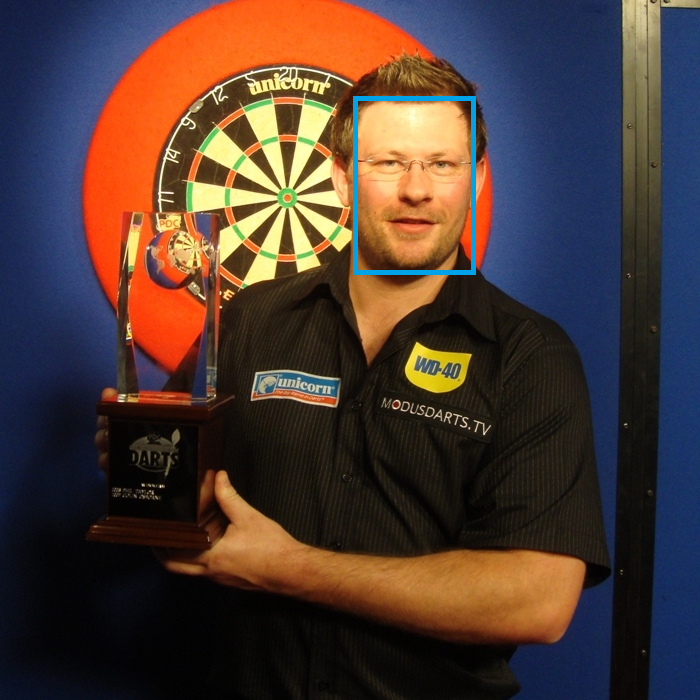
\includegraphics[width=\linewidth]{dart4_faces.png}
          \caption{Annotated dart4.jpg}
        \end{subfigure}
        \begin{subfigure}[b]{0.25\linewidth}
          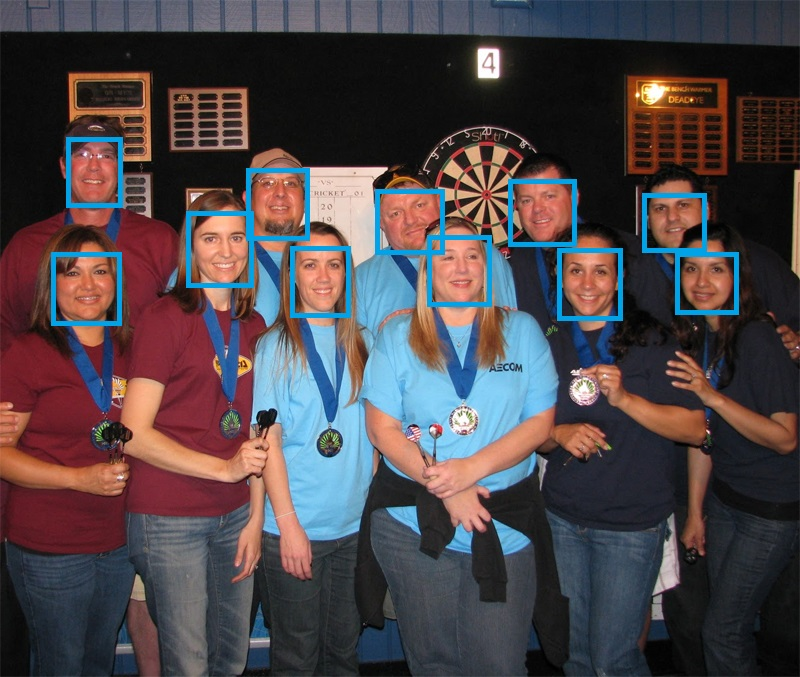
\includegraphics[width=\linewidth]{dart5_faces.png}
          \caption{Annotated dart5.jpg}
        \end{subfigure}
        \begin{subfigure}[b]{0.3\linewidth}
          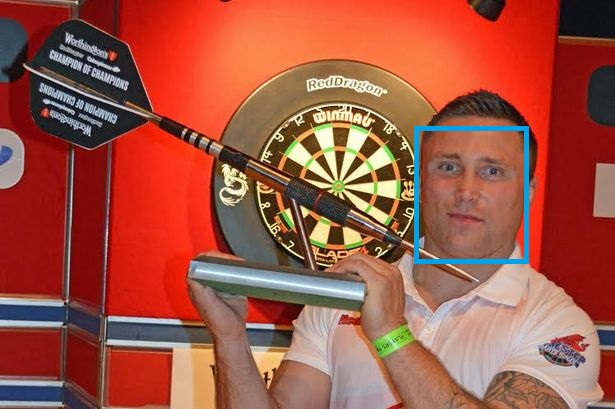
\includegraphics[width=\linewidth]{dart13_faces.png}
          \caption{Annotated dart13.jpg}
        \end{subfigure}
        \begin{subfigure}[b]{0.4\linewidth}
          
\includegraphics[width=\linewidth]{dart14_faces.png}
          \caption{Annotated dart14.jpg}
        \end{subfigure}
        \begin{subfigure}[b]{0.3\linewidth}
          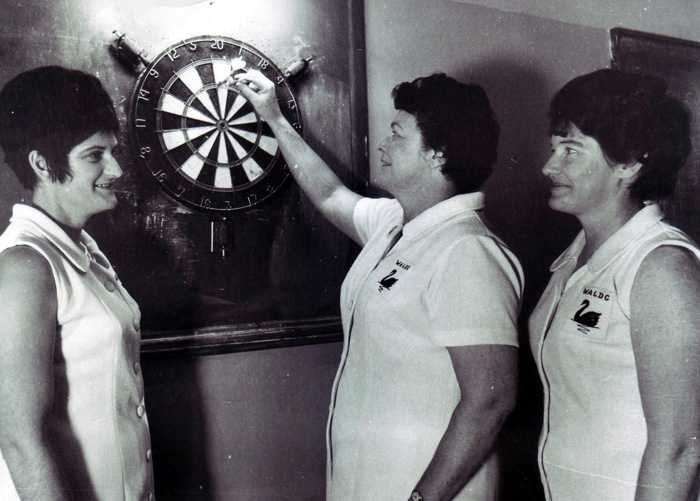
\includegraphics[width=\linewidth]{dart15_faces.png}
          \caption{Annotate dart15.jpg}
        \end{subfigure}
      \end{figure}
    \subsection{True Positive Rate}
      1). The True Positive Rate (TPR) for both face5.jpg and face15.jpg is 100\%. This is despite both images having a lot of objects incorrectly identified as front-on faces, but is to be expected as the TPR does not take into account the number of false positives, and all of the true front-on faces in the images are detected.\\
      2). Either needs to be done manually by comparing annotated ground truth image to test output or by algorithm that detects bounding boxes in both the ground truth and the test output to calculate number of true positives and false negatives. You then have to ensure this algorithm is accurate, although this is an easier problem than face detection.\\
      3). A detection task can always achieve a TPR of 100\% by using an algorithm that classifies every every object within a sub-window as the object you are trying to detect. Then, despite the number of false positives, you would correctly detect all objects within the image, leading to a TPR of 100\%.\\
  \section{Training a Viola-Jones detector}
    \subsection{TPR of the stages detector}
    \begin{figure}
        \centering
        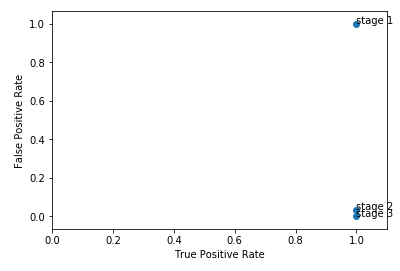
\includegraphics{TPRvsFPR.png}
        \caption{TPR vs FPR of the different stages of the Viola-Jones detector}
        \label{TPRvsFPR}
    \end{figure}
    As more of features are added between the stages the false positive rate decreases whereas the true positive rate does not change. This shows stage one was greatly over identifying objects in the images. As more features are added in stages two and three the false positive rate dramatically drops from \textbf{val in stage 1 to val 2 to val 3}.
    \subsection{Testing the detector}
    \begin{equation}
      F1 score &= 2 * \frac{precision * recall}{precision + recall}\\
      precision &= \frac{true positive}{true positive + false positive}\\
      recall &= \frac{true positives}{true positives + false positives}\\
    \end{equation}\\
    Fix the branches then choose 4 of the pictures to put in this here document. In tabular form calculate the F1 score of all of the images. Whoa, the detection's not great, how does it compare to part a?
\end{document}